\documentclass[9pt]{article}

\usepackage{amsmath}
\usepackage{tcolorbox}
% `parskip` removes indentation for all paragraphs: http://tex.stackexchange.com/a/55016
\usepackage{parskip}
% Allows us to color rows / cols of a table.
% See https://texblog.org/2011/04/19/highlight-table-rowscolumns-with-color/
\usepackage{color, colortbl}

\usepackage{hyperref}
\graphicspath{{images/ps5/}}

\leftmargin=0.25in
\oddsidemargin=0.25in
\textwidth=6.0in
\topmargin=-0.25in
\textheight=9.25in

\definecolor{Gray}{gray}{0.9}

\begin{document}

\begin{center}
  \large\textbf{MIT 18.01 Problem Set 5 Unofficial Solutions}
\end{center}

\begin{tcolorbox}
  \textbf{Q1a)} Suppose that at the beginning of day 0, some time last summer, the temperature in Boston was $y(0) = 65^{\circ}$ Fahrenheit and that over a 50-day period, the temperature increased according to the rule $y'(t) = y(t) / 100$, with time $t$ measured in days. Find the formula for $y$, and draw a graph of temperature on days 3 and 4, $3 <= t <= 5$, and label with the correct day and shade in the regions whose areas represent the average temperature each of the two days.\footnote{The continuous average of a function is $\frac{1}{b - 1} \int_{a}^{b} f(x) dx $ . In this case $b - a = 1$, so the average is the same as the integral. For more, see Notes, AV and Lecture 23.}
\end{tcolorbox}

Based on the rule given, we calculate the temperatures from $t = 0$ to $t = 5$:

\begin{center}
  \begin{tabular}{|c|c|}
    \hline
    \rowcolor{Gray}
    $t$ & $y(t)$ \\ \hline
    0 & 65 \\ \hline
    1 & 65 + 65 / 100 = 65.65 \\ \hline
    2 & 65.65 + 65.65 / 100 = 66.3065 \\ \hline
    3 & 66.3065 + 66.3065 / 100 = 66.969565 \\ \hline
    4 & 66.969565 + 66.969565 / 100 = 67.63926065 \\ \hline
    5 & 67.63926065 + 67.63926065 / 100 = 68.3156532565 \\ \hline
  \end{tabular}
\end{center}

From the formula $y'(t) = y(t) / 100$, we get $\frac{dy}{dt} = \frac{y}{100}$. Then

\begin{align*}
  \frac{dy}{dt} &= \frac{y}{100} \\
  \frac{1}{y} dy &= \frac{1}{100} dt \\
  ln(|y|) &= \frac{1}{100} t + C \\
\end{align*}

Since $y > 0$ and is increasing,

\begin{align*}
  ln(y) &= \frac{1}{100}t + C \\
  y &= e^{\frac{1}{100}t + C} \\
  &= e^{C} \cdot e^{\frac{1}{100}t} \\
  &= Ae^{\frac{1}{100}t}
\end{align*}

At $t = 0, y = 65$. Hence $65 = Ae^{\frac{1}{100} \cdot 0} = A$. Then $ln(y) = 65e^{\frac{1}{100}t}$ \\

Graph:

\begin{center}
  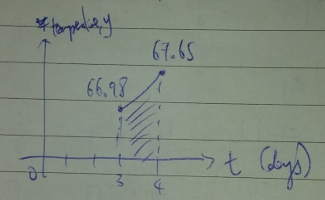
\includegraphics{q1a.jpg}
\end{center}

\end{document}
